\documentclass[11pt]{article}
\usepackage[letterpaper,margin=0.86in]{geometry}
\usepackage{amsmath,amssymb,amsthm,booktabs,array,mathtools}
\usepackage[T1]{fontenc}
\usepackage{lmodern,microtype}
\usepackage[colorlinks=true,linkcolor=blue!45!black,citecolor=blue!45!black,urlcolor=blue!45!black]{hyperref}
\usepackage{xcolor}
\usepackage{graphicx}
\newtheorem{theorem}{Theorem}
\newtheorem{proposition}{Proposition}
\newtheorem{lemma}{Lemma}
\DeclareMathOperator{\ord}{ord}
\DeclareMathOperator{\diag}{diag}
\newcommand{\Z}{\mathbb Z}
\newcommand{\ket}[1]{\lvert #1\rangle}
\newcommand{\bra}[1]{\langle #1\rvert}
\newcommand{\id}{\mathrm{I}}
\title{Recursive Quantum Fourier Circuits for Valuation-Shell States\\[3pt]\large Coherent spectral computation under multiplier symmetry}
\author{Research working draft --- HAD-QFT-04}
\date{27 November 2026}
\begin{document}
\maketitle
\begin{abstract}
The discrete Fourier transform on $\Z/p^n\Z$ preserves the space of functions invariant under multiplication by units. This space has dimension $n+1$; its normalized Fourier matrix is a Ramanujan supercharacter transform. We derive a factorization of this restricted transform into identical adjacent plane rotations and give a binary recursion for the rotation product. For $n+1=2^b$, our explicit circuit uses $5\,2^b+b^2-5b-6$ CNOTs on $b$ qubits without ancillas, or $(b-1)(23b-38)$ CNOTs and at most $b-2$ clean ancillas for $b\ge2$. These counts use arbitrary single-qubit rotations and a six-CNOT Toffoli decomposition. We also derive the character-sector action: a nontrivial multiplicative character of conductor $p^c$ undergoes a shell reversal, conjugation of the character label, and a normalized Gauss phase. An explicit coherent two-sector compiler extends the construction to invariance under units congruent to $1$ modulo $4$. We demonstrate a nested-subgroup hopping Hamiltonian with inexpensive spectral phases, compare against a direct full-register Walsh circuit, and check the emitted circuits using deterministic ideal simulations. The reductions require a native symmetry-adapted encoding; they establish logical quantum resource bounds for promised inputs rather than general QFT or computational speedup. A pilot on an IBM superconducting processor with three and four encoded qubits (128 and 32,768 positions) found $16\%$ and $46\%$ fewer native two-qubit gates for the recursive circuit; measured accuracy was slightly worse at three qubits and moderately better at four qubits, where both circuits were close to the noise limit (Section~\ref{sec:hardware}). A preparation-equivalent compaction (exact) and a bounded-error variant (operator error below $1.7\cdot10^{-3}$) lower the routed CNOT count at five encoded qubits, the transform of ambient dimension $2^{31}$, from 1,122 (Gray) and 468 (recursive) to 296 and 218. On hardware these were the only arms with a clear phase contrast, $0.19$ and $0.31$ for the approximate circuit on two disjoint chains against at most $0.05$ for the recursive circuit, still far below the ideal $1$; at six encoded qubits all contrasts were zero within shot noise (Section~\ref{sec:compact}). Novelty of the circuit factorization requires further literature review.
\end{abstract}

\section{Scope and prior work}
The quantum Fourier transform (QFT) is a coherent change of basis used in period finding, phase estimation and spectral algorithms. General-purpose approximate QFT circuits can achieve substantially better scaling than an elementary quadratic construction; see, for example, Nam, Su and Maslov \cite{nam} and the recursive construction proposed by Shah \cite{shah}. Our resource comparisons concern a restricted input/output interface. A full-register approximate QFT and an encoded restricted QFT solve different tasks.

The present approach arose from integer autocorrelation certificates for group-developed Hadamard matrices, where common multiplier symmetries and Chinese remainder decompositions reduce both the sign search and the Fourier verification. The normalized Ramanujan matrix and its factorization over coprime moduli are established mathematics \cite{fowler,brumbaugh}. We use those facts to design a circuit that exploits the matrix's special structure. Hierarchical Laplacians and finite models of $p$-adic quantum walks supply a physical setting for symmetry-preserving dynamics \cite{bendikov,zuniga}. We distinguish the circuit derivations and tests below from any claim of literature priority.

Let $F_N$ denote the positive-exponent unitary Fourier transform,
\begin{equation}
 (F_N)_{yx}=N^{-1/2}\exp(2\pi i xy/N).
\end{equation}
If $u$ is a unit modulo $N$, write $M_u\ket{x}=\ket{ux}$. Then $F_N M_u=M_{u^{-1}}F_N$. For a subgroup $K$ of units, the invariant subspace is spanned by the normalized orbit vectors $\ket{O}=|O|^{-1/2}\sum_{x\in O}\ket{x}$. Write $B_K$ for the isometric embedding of the orbit register and $Q_K=B_K^*F_N B_K$. The intertwining identity is $F_N B_K=B_K Q_K$. If $-1\in K$, $F_N^2=M_{-1}$ implies that $Q_K$ is an involution; the Fourier entries paired by inversion also make $Q_K$ real and symmetric.

For pairwise coprime factors $m_i$ with $N=\prod_i m_i$, use time labels $x_i=x\bmod m_i$ and dual frequency labels $k_i=(N/m_i)^{-1}k\bmod m_i$. The character kernel separates over the factors. When the multiplier group is a direct product, the normalized orbit transform is a tensor product in these two label systems. Full unit invariance at $N=\prod_i p_i^{e_i}$ has dimension $\prod_i(e_i+1)=\tau(N)$. The factorization is assumed known. It is not an algorithm for finding the factorization.

\section{Prime-power shell transform}
For $N=p^n$, the unit group acts transitively on each set of fixed additive order. Define $S_0=\{0\}$, and for $1\le j\le n$, put
\begin{equation}
 S_j=\{p^{n-j}a: a\in (\Z/p^j\Z)^\times\},\qquad w_j=(p-1)p^{j-1},\quad w_0=1.
\end{equation}
The normalized orbit vector is $\ket{j}_{\rm phys}=w_j^{-1/2}\sum_{x\in S_j}\ket{x}$. The $n+1$ abstract shell labels are denoted $\ket{j}$. They need not be represented by physical position labels at any stage of the encoded algorithm.

The Ramanujan sum over units of a prime power vanishes for conductor $p^r$ with $r\ge2$, is $-1$ at conductor $p$, and is the unit count at the trivial character. In the shell basis this gives the known normalized matrix
\begin{equation}\label{eq:q}
 Q_{ij}=\sqrt{\frac{w_i w_j}{p^n}}\begin{cases}
 1,& i=0\text{ or }j=0\text{ or }i+j\le n,\\
 -1/(p-1),& i,j>0,\ i+j=n+1,\\
 0,&\text{otherwise}.
 \end{cases}
\end{equation}
Set $c=\sqrt{(p-1)/p}$, $d=1/\sqrt p$. Let $R$ reverse the labels $0,\ldots,n$ and let $G_j$ be the identity except on $(j,j+1)$, where its matrix is $\left(\begin{smallmatrix}c&d\\-d&c\end{smallmatrix}\right)$.
\begin{theorem}[Adjacent rotations]\label{thm:adj}
In the shell basis, $Q R=G_0G_1\cdots G_{n-1}$.
\end{theorem}
\begin{proof}
Write $v_j=\sum_{i=0}^j\sqrt{w_i/p^j}\ket{i}$. Then $v_0=\ket{0}$ and $v_j=d v_{j-1}+c\ket{j}$. Induction gives $G_0\cdots G_{j-1}\ket{j}=v_j$. For $j<n$ the resulting column is $c v_j-d\ket{j+1}$; the final column is $v_n$. Substituting the weights in (\ref{eq:q}) gives exactly the reversed columns of $Q$. All products here are exact real matrix identities.
\end{proof}
A direct circuit for each two-level rotation uses a Gray-coded shell register and a uniformly controlled rotation. If $n+1=2^b$ and $b\ge2$, it needs $n2^{b-1}$ CNOTs. We next exploit the order and equal angles of the rotations to lower this count.

\section{Binary recursive compilation}
\label{sec:recursive}
Let $W_D$ denote the rotation product in Theorem~\ref{thm:adj} on $D$ levels, with $W_1=1$. For $D=2L$, partition the labels into two equal contiguous halves. The rotations wholly within the two halves form copies of $W_L$; the single boundary rotation acts between $\ket{0,L-1}$ and $\ket{1,0}$. Thus
\begin{equation}\label{eq:factor}
 W_{2L}=(W_L\oplus\id)G_{L-1}(\id\oplus W_L)
 = (\id_2\otimes W_L)(\id\oplus W_L^T)G_{L-1}(\id\oplus W_L).
\end{equation}
The right half of the conjugated rotation uses $g_L=W_L^T\ket{0}$. From the column formula above,
\begin{equation}\label{eq:g}
 g_L=c\ket{0}+cd\ket{1}+\cdots+cd^{L-2}\ket{L-2}+d^{L-1}\ket{L-1}.
\end{equation}
The vector is normalized by $c^2=1-d^2$. Our binary conditional-mass preparation uses the standard state-loading approach of Grover and Rudolph \cite{grover} and uniformly controlled rotations \cite{mottonen}. Let $P_L$ be a unitary satisfying
\begin{equation}
 P_L\ket{0,0}=\ket{0,L-1},\qquad P_L\ket{1,0}=\ket{1,g_L}.
\end{equation}
It can preserve the leading binary digit. Let $C_L$ apply $R_y(-2\arcsin d)$ to that digit conditioned on every remaining bit being zero, with $R_y(\theta)=\left(\begin{smallmatrix}\cos(\theta/2)&-\sin(\theta/2)\\\sin(\theta/2)&\cos(\theta/2)\end{smallmatrix}\right)$. The two conjugations act identically on the affected plane and as identity on its orthogonal complement. Equation (\ref{eq:factor}) therefore gives the recursion
\begin{equation}\label{eq:rec}
 \boxed{ W_{2L}=(\id_2\otimes W_L)P_L C_L P_L^\dagger. }
\end{equation}
Only one copy of the smaller quantum circuit is required: its action on the lower bits is unconditional.

\paragraph{Preparing $g_L$.} Let $L=2^r$, and generate the lower bits from most to least significant. When preparing bit $k=0,\ldots,r-1$, set $z=d^{2^{r-1-k}}$. If the prefix is all ones (including the empty prefix), the remaining conditional state is again a truncated geometric state. Its probability of the right half is $z^2$. Otherwise the conditional amplitudes are proportional to a geometric sequence, with ratio of right-half to left-half norms equal to $z$. Consequently the rotation angles are $2\arcsin z$ on the all-ones prefix and $2\arctan z$ on other prefixes. On the leading-zero branch, $P_L$ instead flips all lower bits, mapping the zero label to $L-1$. These conditions specify a full unitary implementation, not just a state map: we use the prescribed controlled rotations on arbitrary inputs and their actual inverse in (\ref{eq:rec}).

\begin{theorem}[Resource counts]\label{thm:cost}
Suppose $n=2^b-1$, $b\ge1$. With arbitrary single-qubit rotations, all-to-all logical connections, and a six-CNOT exact Toffoli decomposition, the following CNOT counts implement the shell QFT:
\begin{align}
 C_{\rm noanc}(b)&=5\,2^b+b^2-5b-6,\\
 C_{\rm clean}(b)&=(b-1)(23b-38).
\end{align}
The first circuit uses $b$ qubits. The second uses $b+\max(0,b-2)$ qubits, with clean work bits returned to zero. Total elementary gate counts have order $O(2^b)$ and $O(b^2)$, respectively. A hybrid may take the cheaper construction at each recursive level.
\end{theorem}
\begin{proof}
In a level with $r$ lower bits, the left-branch complement in $P_L$ uses $r$ CNOTs. For the right branch, a Gray-cycle multiplexer for bit $k$ has $k+1$ controls including the leading digit, so it uses $2^{k+1}$ CNOTs and the same number of rotations. The total for $P_L$ is $r+2^{r+1}-2$. The middle rotation $C_L$ costs $2^r$ CNOTs by the same multiplexer. With the inverse preparation included, this level costs $5\,2^r+2r-4$ CNOTs.

With clean workspace, compute the prefix-AND flags during preparation and uncompute them in reverse order after the last rotation. Every prefix is a predicate of already-prepared bits; later rotations never change those bits. The first right-branch rotation is singly controlled. Each subsequent bit uses one rotation controlled by the leading bit plus a correction controlled by the prefix flag. This gives $2r-1$ singly controlled rotations and $2(r-1)$ Toffolis in $P_L$. For $C_L$, flip the lower bits, compute their conjunction, rotate the leading bit once, and uncompute. Its cost is one controlled rotation and $2(r-1)$ Toffolis. In total, this level uses $2r$ direct CNOTs, $4r-1$ controlled rotations (two CNOTs each) and $6(r-1)$ Toffolis. Hence its cost is $46r-38$. The $r-1$ work bits can be reused at later levels. The bottom $W_2$ is one rotation with no CNOT, and $R$ is bitwise complement, requiring only $b$ X gates. Summing over $r=1,\ldots,b-1$ proves the formulas. The other elementary gates have the same asymptotic bounds.
\end{proof}
The equal-size recursion has been proved for the family $n+1=2^b$. General $n$ still has the shell matrix and adjacent rotation product, but a comparably efficient padding or unequal-size recursion remains to be studied. Rotation angles are exact analytic specifications; actual hardware or finite gate-set approximations introduce synthesis error. If $M$ ideal elementary rotations are approximated with operator error at most $\eta/M$ each, telescoping gives total operator error at most $\eta$. We do not report synthesized T counts for arbitrary rotations.

\begin{table}[htbp]
\centering\small
\caption{Logical CNOT counts for a single restricted QFT. The original full position register has $n$ bits when $p=2$. ``Old'' is the direct Gray-cycle shell compiler; ``hybrid'' selects a lower-cost construction per recursion level. Counts at large $n$ follow from circuit generation and Theorem~\ref{thm:cost}, rather than full position-space simulation.}
\begin{tabular}{rrrrrr}
\toprule
$n$ & $b$ & Old & No ancilla & Hybrid & Hybrid wires\\
\midrule
7 & 3 & 28 & 28 & 28 & 3\\
15 & 4 & 120 & 70 & 70 & 4\\
31 & 5 & 496 & 154 & 154 & 5\\
63 & 6 & 2,016 & 320 & 320 & 6\\
127 & 7 & 8,128 & 648 & 558 & 12\\
255 & 8 & 32,640 & 1,298 & 842 & 14\\
1,023 & 10 & 523,776 & 5,164 & 1,548 & 18\\
4,095 & 12 & 8,386,560 & 20,558 & 2,438 & 22\\
\bottomrule
\end{tabular}
\end{table}

\section{Nontrivial character sectors and partial symmetry}
Let $\chi$ be a nontrivial multiplicative character of the unit group of $\Z/p^n\Z$, induced by a primitive character modulo $p^a$ with $1\le a\le n$ (its conductor is $p^a$). For $j\ge a$ define
\begin{equation}
 \ket{j,\chi}=\frac{1}{\sqrt{w_j}}\sum_{u\in(\Z/p^j\Z)^\times}\chi(u)\ket{p^{n-j}u}.
\end{equation}
These vectors span the character sector in which multiplier $v$ acts by $\chi(v)^{-1}$. At each shell with $j<a$, the stabilizer includes units on which $\chi$ is nontrivial, so no vector of that character type exists there.
\begin{theorem}[Conductor-resolved transform]\label{thm:char}
Define $\gamma_\chi=p^{-a/2}\sum_{u\in(\Z/p^a\Z)^\times}\chi(u)e^{2\pi i u/p^a}$. For $a\le j\le n$,
\begin{equation}\label{eq:char}
 F_{p^n}\ket{j,\chi}=\gamma_\chi\ket{n+a-j,\overline{\chi}},\qquad |\gamma_\chi|=1.
\end{equation}
\end{theorem}
\begin{proof}
On a nonzero output shell $\ell$ write $y=p^{n-\ell}v$ with $v$ a unit. The unnormalized sum in the Fourier coefficient has additive conductor $p^{j+\ell-n}$ if $j+\ell>n$, and is a constant additive phase otherwise. If the additive conductor is smaller than $p^a$, summing over the character's nontrivial kernel of reduction gives zero. If it is greater, the character is constant on the lifts of a residue modulo $p^a$, while the geometric sum of additive phases over those lifts is zero. At equality $j+\ell=n+a$, the sum is $p^{j-a}\overline\chi(v)$ times the Gauss sum modulo $p^a$. Converting to normalized shell vectors multiplies this sum by $\sqrt{w_\ell}/(p^{n/2}\sqrt{w_j})$, giving (\ref{eq:char}). The zero output coordinate vanishes since $\chi$ is nontrivial. Unitarity now yields $|\gamma_\chi|=1$.
\end{proof}
For a known fixed character, the compressed transform is a reversal of $n-a+1$ labels, together with a relabeling of the output character. If that length is a power of two, the reversal is bitwise complement. The Gauss phase is global only for a fixed, uncontrolled sector. A coherent superposition of sectors must retain their relative phases. These phases and the required encoding need not be cheap for arbitrary characters of growing conductor.

For $1\le s\le n$, define $K_s=\{u:u\equiv1\pmod {p^s}\}$. Its invariant subspace is the direct sum of the trivial sector and all characters of conductor at most $p^s$. Counting orbits on shells gives
\begin{equation}
 \dim\mathcal H^{K_s}=p^s+(n-s)\varphi(p^s).
\end{equation}
This broadens the promise to more than fully unit-invariant states; for fixed $p,s$ the dimension still grows linearly with $n$.

\paragraph{An explicit two-sector circuit.} For $p=2,s=2$ there are the trivial character and $\chi_4(u)=(-1)^{(u-1)/2}$, with normalized Gauss phase $i$. The dimension is $2n$. Use a character flag and an absolute $b$-bit shell label, where flag 1 is valid for $j\ge2$. A flag-controlled version of Theorem~\ref{thm:cost} implements the trivial block; the other block maps $j\mapsto n+2-j\equiv 1-j\pmod{2^b}$ and applies phase $i$ to the flag. This permutation is complement followed by addition of two modulo $2^b$. Controlled increment of the upper $b-1$ bits uses a reversible carry chain whose flags are uncomputed before their source bits change. Adding one control to each gate of the clean recursion costs at most a constant number of gates using one scratch bit. The result has $O(b^2)$ logical gates and $2b$ total wires for $b\ge2$, with workspace restored. Unused labels are given a unitary extension. The code implements this coherent circuit; its constants are larger than those for the single-sector compiler.

\section{Application: coherent hierarchical hopping}
Let $H_j$ be the additive subgroup of order $p^j$ in $\Z/p^n\Z$, and define the orthogonal projector
\begin{equation}
 (A_j f)(x)=p^{-j}\sum_{h\in H_j} f(x+h).
\end{equation}
In Fourier coordinates, $A_j$ is the indicator of $H_j^\perp$; on shell $r$ it has eigenvalue $\mathbf1_{r\le n-j}$. The uniform-weight Hamiltonian $H=\sum_{j=1}^n(\id-A_j)$ therefore has eigenvalue $r$ on Fourier shell $r$. More general real weights give eigenvalues $E_r=\sum_{j>n-r}w'_j$. The fast phase circuit below is for uniform weights; a general table of eigenvalues has its own implementation cost.

In the trivial sector, the uniform Hamiltonian evolves as
\begin{equation}
 U(t)=Q^*\diag_{r}(e^{-itr})Q.
\end{equation}
The binary shell index is a weighted sum of bits, so the diagonal is a tensor product of $b$ phase gates. A position potential depending on shell index is diagonal in the original shell basis. In particular, a linear potential gives another $b$ phase gates. Alternating exact hopping and such potential steps stays in the same native compressed register. This supplies a coherent use case, where a measurement-only Fourier sampler would lose the required phase information. A localized origin initial state is simply the all-zero shell state; any shell basis initial state also has a direct encoding. A physical position readout from a shell probability sample may be obtained by drawing a uniform member of that shell.

For $p=2$ a stronger full-register baseline avoids the usual QFT altogether. Translation by the subgroup of size $2^j$ permutes the high $j$ bits while preserving the other bits; averaging projects the high bits onto the tensor product $\ket{+}^{\otimes j}$. Thus a tensor product of Hadamards diagonalizes all the $A_j$. Compute the all-zero prefix predicates with $n-1$ clean bits, apply the phases, and uncompute. This particular circuit uses $2(n-1)$ Toffolis, or $12(n-1)$ CNOTs, with $2n-1$ total wires. It is a direct coherent baseline and need not be optimal. Table~\ref{tab:app} includes this cost rather than assigning two generic QFTs to the full algorithm.
\begin{table}[htbp]
\centering\small
\caption{Uniform hierarchical hopping: one coherent time step, $p=2$. Both circuits have diagonal phase costs in addition to the CNOT counts.}\label{tab:app}
\begin{tabular}{rrrrr}
\toprule
Original bits $n$ & Full Walsh wires & Full Walsh CX & Shell wires & Shell CX\\
\midrule
7 & 13 & 72 & 3 & 56\\
15 & 29 & 168 & 4 & 140\\
31 & 61 & 360 & 5 & 308\\
127 & 253 & 1,512 & 12 & 1,116\\
255 & 509 & 3,048 & 14 & 1,684\\
1,023 & 2,045 & 12,264 & 18 & 3,096\\
\bottomrule
\end{tabular}
\end{table}

\section{Validation, Hadamard case study, and scope limits}
All reported new checks are local ideal CPU simulations, using double-precision arithmetic for quantum amplitudes. The Python reference independently evaluates (\ref{eq:q}) and directly evolves the chronological gates. A separate direct simulator verifies the elementary controlled-rotation and Toffoli decompositions. The audit includes the following coverage:
\begin{center}\small
\begin{tabular}{p{0.60\linewidth}r}
\toprule
Check & Count or maximum error\\
\midrule
Recursive compilation settings & 58\\
Basis columns and random complex test vectors & 1,184\\
Maximum compiled amplitude error & $7.33\cdot10^{-15}$\\
Maximum workspace leakage norm & $2.59\cdot10^{-15}$\\
Hierarchical hopping parameter settings & 8\\
Full FFT evolution amplitude error & $1.02\cdot10^{-15}$\\
Dense Hamiltonian exponential error (small cases) & $3.33\cdot10^{-15}$\\
Six-step alternating evolution error & $1.23\cdot10^{-15}$\\
Nontrivial character sectors enumerated & 490\\
Nontrivial shell columns checked by FFT & 769\\
Maximum character transform error & $4.49\cdot10^{-16}$\\
Two-sector compiler basis columns & 248\\
Maximum two-sector compiler error & $4.45\cdot10^{-16}$\\
\bottomrule
\end{tabular}
\end{center}
Full direct FFT references for the two-sector compiler cover $N=8,128,32768$. For the single-sector compiler, all columns are simulated through $64$ shell levels for each $p\in\{2,3,5,7\}$ in both principal modes, with larger binary tests and one fully elementary decomposition. The full underlying position vector is not generated at the largest represented sizes. A repeat audit produced byte-identical JSON and text receipts. The code emits OpenQASM 3. The ideal simulations above do not include routing or noise; a limited hardware pilot is reported in Section~\ref{sec:hardware}, while fault-tolerant synthesis remains future work.

The original application was a cyclic Hadamard-core problem at order 2396. Its length-598 core admits a candidate order-eight multiplier group with CRT factors of dimensions $2,13,23$ and orbit dimensions $2,4,12$. The earlier ideal-simulation study used a seven-wire encoding of these 96 orbit labels, with a 140-CNOT real cosine-sine compiler; it also checked exact modular autocorrelation certificates. This is an illustration of the more general orbit restriction. It does not construct a new Hadamard matrix or establish the existence of a length-598 core in that family. The new prime-power recursion relies on the special shell matrix rather than applying to arbitrary multiplier orbit transforms.

\paragraph{Approximate symmetry.} With orbit projection $P$ and a normalized input $\psi$, let $\epsilon=\|(\id-P)\psi\|^2$. If $\epsilon<1$, its normalized projection has squared fidelity $1-\epsilon$ with $\psi$. Every common unitary continuation preserves this fidelity, and every measurement has total-variation error at most $\sqrt\epsilon$. In a symmetry-preserving circuit the projected branch can be represented in the smaller register throughout. This guarantee presumes that the encoded projected input is available. Neither projection success nor a general encoder is free. Additional symmetry-breaking operations require a separate error analysis.

\paragraph{Limits on general QFT acceleration.} For a phase ramp $\psi_k(x)=N^{-1/2}e^{2\pi i kx/N}$, the projection onto unit-invariant states retains squared norm $1/|O(k)|$: Fourier transforms the ramp to a basis vector at $-k$, and the projector commutes with $F_N$. For a unit $k$, this is $1/\varphi(N)$, exponentially small in the binary position width for prime powers. Our audit verifies the identity on 237 phase ramps. Standard phase estimation and period-finding registers have no general invariant-input promise. A complete character-basis decomposition of the unrestricted QFT would also need a coherent change of basis from position labels and implementation of conductor-dependent phases. Their costs have not been bounded here.

The invariant dynamics can be classically simulated with $O(n)$ amplitudes, and the adjacent rotation product itself can be evaluated classically in $O(n)$ arithmetic operations. We therefore make no quantum-advantage claim. The result is a reduction in encoded logical circuit resources for a symmetry-preserving quantum computation, including coherent access by a larger quantum algorithm. Comparisons must account for state preparation, conversion, phase oracles, desired output, approximation error and hardware connectivity.

\section{Hardware evaluation on IBM Quantum}\label{sec:hardware}
\paragraph{Question and scope.} We ask whether the recursive binary shell QFT preserves coherent Fourier interference more accurately than the earlier Gray-code shell QFT while requiring fewer hardware resources. The comparison is confined to the symmetry-adapted input space: the registers hold $b$-qubit encodings of the $2^b$ shell labels, and both circuits implement the same $2^b\times2^b$ shell transform $Q$, represented by $N=2^{2^b-1}$ positions ($b=3$: $128$; $b=4$: $32{,}768$). The Gray arm is the earlier circuit followed by the Gray-to-binary label conversion, so that both arms use the same logical coordinates. The experiment says nothing about a general QFT, state preparation of position-space inputs, or computational advantage.

\paragraph{Protocol.} The campaign was a prospective exploratory pilot, executed on 27 November 2026 on \texttt{ibm\_kingston} through Qiskit Runtime (Qiskit 2.6.2, \texttt{qiskit-ibm-runtime} 0.52.0), with the compiled plan hash recorded before each submission and owner authorization of that hash. Each stage was one Sampler job of 384 shots per circuit with a fixed shuffled order, a calibration-selected linear physical chain, no dynamical decoupling and optimization level zero (so that the routed gate sequences, including nearest-neighbor CNOT bridges, are preserved). The roster was fixed in advance: 30 circuits for $b=3$ and 38 for $b=4$. For four input probes (the first and last basis states and the real and imaginary two-shell superpositions) each arm was measured in the computational basis and in the $X$ (real) or $Y$ (imaginary) basis that exposes interference, for two coherent probes each arm also ran an inverse-transform echo, prep-only echoes isolate the preparation, and every basis state was prepared and read out as a SPAM control. All metrics use raw counts; no readout mitigation is used in any reported number. The $b=3$ stage used physical qubits $[38,49,48]$ and the $b=4$ stage used $[148,149,150,151]$, both under the device calibration of 27 November 2026, 11:57 UTC, which was unchanged at submission; the two arms always shared the same chain and the same job. Job identifiers are \texttt{dc4n8nmq4uuc73a94qa0} ($b=3$, plan hash \texttt{927978a9083f}) and \texttt{dc4nal6q4uuc73a94sm0} ($b=4$, plan hash \texttt{c4a993303704}). The two jobs were charged 5 and 6 QPU seconds by IBM, 11 in total against the 30-second reservation; the account had 354 of 600 seconds remaining afterwards.

\paragraph{Metrics and uncertainty.} For each circuit the empirical distribution $\hat p$ is compared with the ideal distribution $q$ by total variation $\mathrm{TV}=\tfrac12\|\hat p-q\|_1$ and Hellinger fidelity $F_H=(\sum\sqrt{\hat pq})^2$. The paired difference $\Delta=\mathrm{TV}_{\rm Gray}-\mathrm{TV}_{\rm rec}$ is positive when the recursive circuit is closer to ideal. Intervals are 95\% multinomial bootstrap intervals computed from the observed counts and capture finite-shot variation only. They do not include drift, calibration error, or the variation in how the compiled circuits sample correlated hardware noise, which is the quantity of interest here, so they must not be read as hypothesis tests of the hardware effect. Two reference levels bound what is measurable. The ideal-sampling floor is the mean TV a perfect device would show with 384 shots ($0.040$ for $b=3$, $0.052$ for $b=4$). The uniform-noise reference is the TV between the ideal distribution and the uniform distribution, the value a fully depolarized readout would give ($0.445$ and $0.571$). The Hellinger fidelity of the $b=4$ data is correspondingly low. Coherent-readout metrics use the $X$/$Y$-basis rows; we also report the parity $\langle\sigma^{\otimes b}\rangle$ of those readouts against its ideal value.

\begin{table}[htbp]\centering\small
\caption{Stage $b=3$ compiled resources for the core transform on ibm\_kingston (physical qubits [38, 49, 48]). Counts are IBM ISA native gates at optimization level 0; duration is the calibrated schedule length of one shot.}
\label{tab:hw-res-b3}\begin{tabular}{lrr}\toprule Quantity & Gray shell & Recursive\\\midrule
Logical CNOT (with label conversion) & 32 & 28\\
Nearest-neighbor CNOT after bridging & 62 & 52\\
Native two-qubit gates & 62 & 52\\
Two-qubit depth & 62 & 52\\
Circuit depth & 395 & 360\\
Duration ($\mu$s) & 9.66 & 9.08\\
\bottomrule\end{tabular}\end{table}

\begin{table}[htbp]\centering\small
\caption{Stage $b=3$ paired forward-transform results, raw counts, 384 shots per circuit. $\Delta=\mathrm{TV}_{\rm Gray}-\mathrm{TV}_{\rm rec}$ (positive favors the recursive circuit); brackets are 95\% multinomial bootstrap intervals from finite shots only. The ideal-sampling floor is the mean TV a perfect device would show at this shot count.}
\label{tab:hw-pairs-b3}\begin{tabular}{llrrrcrr}\toprule Probe & Basis & TV Gray & TV rec & $\Delta$ & 95\% interval & $F_H$ Gray & $F_H$ rec\\\midrule
imag & Y & 0.137 & 0.130 & +0.007 & [-0.062,+0.065] & 0.976 & 0.975\\
imag & Z & 0.069 & 0.111 & -0.042 & [-0.094,+0.026] & 0.992 & 0.983\\
last & X & 0.122 & 0.135 & -0.013 & [-0.065,+0.049] & 0.887 & 0.877\\
last & Z & 0.102 & 0.117 & -0.016 & [-0.068,+0.023] & 0.898 & 0.880\\
plus & X & 0.187 & 0.220 & -0.033 & [-0.103,+0.033] & 0.937 & 0.916\\
plus & Z & 0.064 & 0.113 & -0.050 & [-0.100,+0.015] & 0.987 & 0.977\\
zero & X & 0.108 & 0.163 & -0.056 & [-0.109,+0.007] & 0.943 & 0.919\\
zero & Z & 0.115 & 0.109 & +0.005 & [-0.052,+0.073] & 0.968 & 0.979\\
\midrule
Mean & & 0.113 & 0.137 & -0.025 & [-0.041,-0.001] & 0.949 & 0.938\\
Ideal floor & & 0.040 & 0.040 & & & &\\
\bottomrule\end{tabular}\end{table}

\begin{table}[htbp]\centering\small
\caption{Stage $b=3$ inverse-transform echoes and controls (ideal return probability 1; 95\% Wilson intervals). Prep-only rows contain the state preparation and its inverse without the transform.}
\label{tab:hw-echo-b3}\begin{tabular}{lrrc}\toprule Circuit & Probe & Return probability & 95\% interval\\\midrule
gray & plus & 0.607 & [0.557,0.654]\\
recursive & plus & 0.523 & [0.473,0.573]\\
prep & plus & 0.932 & [0.903,0.953]\\
gray & imag & 0.542 & [0.492,0.591]\\
prep & imag & 0.927 & [0.897,0.949]\\
recursive & imag & 0.581 & [0.531,0.629]\\
\midrule
SPAM, mean correct readout & all 8 basis states & 0.988 & min 0.977\\
\bottomrule\end{tabular}\end{table}

\begin{table}[htbp]\centering\small
\caption{Stage $b=4$ compiled resources for the core transform on ibm\_kingston (physical qubits [148, 149, 150, 151]). Counts are IBM ISA native gates at optimization level 0; duration is the calibrated schedule length of one shot.}
\label{tab:hw-res-b4}\begin{tabular}{lrr}\toprule Quantity & Gray shell & Recursive\\\midrule
Logical CNOT (with label conversion) & 126 & 70\\
Nearest-neighbor CNOT after bridging & 368 & 200\\
Native two-qubit gates & 368 & 200\\
Two-qubit depth & 335 & 192\\
Circuit depth & 2008 & 1093\\
Duration ($\mu$s) & 41.41 & 24.29\\
\bottomrule\end{tabular}\end{table}

\begin{table}[htbp]\centering\small
\caption{Stage $b=4$ paired forward-transform results, raw counts, 384 shots per circuit. $\Delta=\mathrm{TV}_{\rm Gray}-\mathrm{TV}_{\rm rec}$ (positive favors the recursive circuit); brackets are 95\% multinomial bootstrap intervals from finite shots only. The ideal-sampling floor is the mean TV a perfect device would show at this shot count.}
\label{tab:hw-pairs-b4}\begin{tabular}{llrrrcrr}\toprule Probe & Basis & TV Gray & TV rec & $\Delta$ & 95\% interval & $F_H$ Gray & $F_H$ rec\\\midrule
imag & Y & 0.312 & 0.315 & -0.003 & [-0.063,+0.071] & 0.846 & 0.864\\
imag & Z & 0.430 & 0.412 & +0.018 & [-0.039,+0.083] & 0.647 & 0.677\\
last & X & 0.516 & 0.378 & +0.138 & [+0.065,+0.206] & 0.465 & 0.614\\
last & Z & 0.531 & 0.586 & -0.055 & [-0.122,+0.016] & 0.391 & 0.392\\
plus & X & 0.477 & 0.532 & -0.055 & [-0.123,+0.010] & 0.689 & 0.593\\
plus & Z & 0.481 & 0.385 & +0.096 & [+0.031,+0.156] & 0.602 & 0.723\\
zero & X & 0.551 & 0.412 & +0.139 & [+0.079,+0.197] & 0.560 & 0.707\\
zero & Z & 0.529 & 0.513 & +0.016 & [-0.052,+0.086] & 0.547 & 0.579\\
\midrule
Mean & & 0.478 & 0.441 & +0.037 & [+0.013,+0.061] & 0.593 & 0.644\\
Ideal floor & & 0.052 & 0.052 & & & &\\
\bottomrule\end{tabular}\end{table}

\begin{table}[htbp]\centering\small
\caption{Stage $b=4$ inverse-transform echoes and controls (ideal return probability 1; 95\% Wilson intervals). Prep-only rows contain the state preparation and its inverse without the transform.}
\label{tab:hw-echo-b4}\begin{tabular}{lrrc}\toprule Circuit & Probe & Return probability & 95\% interval\\\midrule
gray & imag & 0.083 & [0.060,0.115]\\
recursive & imag & 0.039 & [0.024,0.063]\\
gray & plus & 0.065 & [0.044,0.094]\\
recursive & plus & 0.078 & [0.055,0.109]\\
prep & imag & 0.732 & [0.685,0.774]\\
prep & plus & 0.758 & [0.713,0.798]\\
\midrule
SPAM, mean correct readout & all 16 basis states & 0.981 & min 0.961\\
\bottomrule\end{tabular}\end{table}


\begin{figure}[htbp]\centering
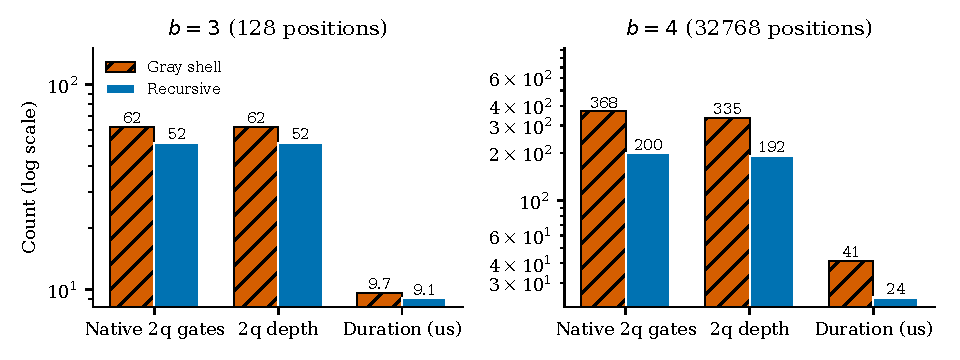
\includegraphics[width=0.98\linewidth]{figures/hw_resources.pdf}
\caption{Compiled resources of the core transform (log scale): native two-qubit gates, two-qubit depth and calibrated duration of one shot, for the Gray and recursive circuits. These are properties of the compiled circuits, not of the measured outcomes.}\label{fig:hw-resources}
\end{figure}

\begin{figure}[htbp]\centering
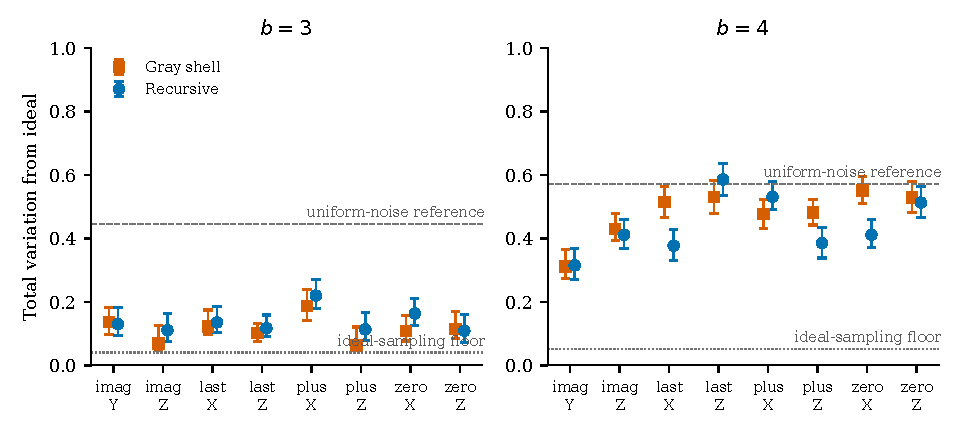
\includegraphics[width=0.98\linewidth]{figures/hw_paired_tv.pdf}
\caption{Total variation distance from the ideal distribution for each paired circuit (raw counts; bars are 95\% finite-shot bootstrap intervals). Dotted line: ideal-sampling floor. Dashed line: uniform-noise reference. For $b=4$ most points lie between 0.3 and 0.6, close to the dashed line.}\label{fig:hw-tv}
\end{figure}

\begin{figure}[htbp]\centering
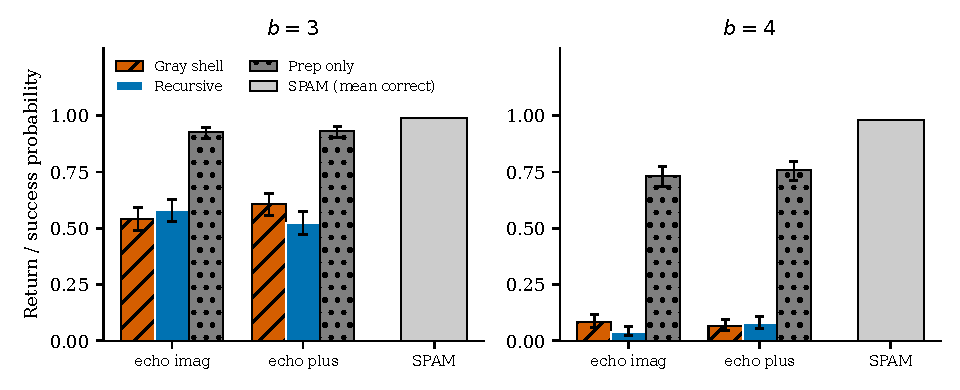
\includegraphics[width=0.98\linewidth]{figures/hw_echo.pdf}
\caption{Inverse-transform echo return probabilities, the corresponding prep-only echoes and the SPAM control (95\% Wilson intervals). The $b=4$ transform echoes are at the level of a uniform distribution over 16 outcomes ($0.0625$).}\label{fig:hw-echo}
\end{figure}

\begin{figure}[htbp]\centering
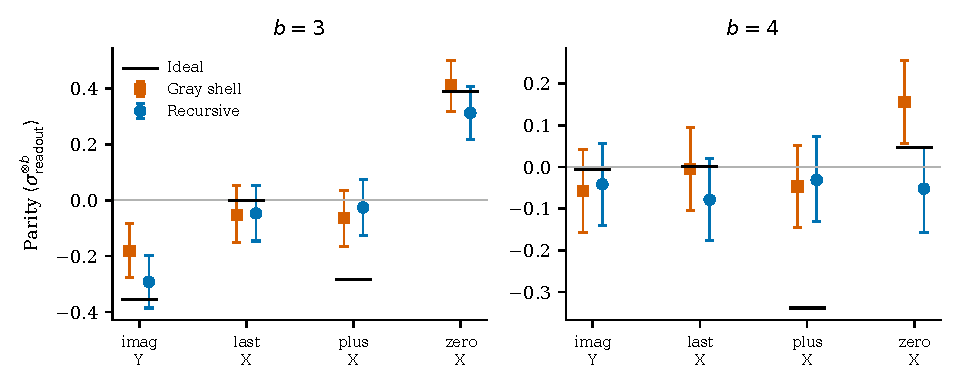
\includegraphics[width=0.98\linewidth]{figures/hw_coherence.pdf}
\caption{Parity of the interference readouts ($X$ for the real probes, $Y$ for the imaginary probe) against the ideal value (black bars). Error bars are 95\% finite-shot bootstrap intervals.}\label{fig:hw-coherence}
\end{figure}

\paragraph{Resources.} The compiled recursive circuits are smaller at both sizes (Table~\ref{tab:hw-res-b3} and \ref{tab:hw-res-b4}, Figure~\ref{fig:hw-resources}). At $b=3$ the core transform needs $52$ native two-qubit gates versus $62$ ($-16\%$), two-qubit depth $52$ versus $62$, total depth $360$ versus $395$ and $9.08$ versus $9.66\,\mu$s of schedule. At $b=4$ the counts are $200$ versus $368$ ($-46\%$) native two-qubit gates, depth $1093$ versus $2008$ and $24.3$ versus $41.4\,\mu$s ($-41\%$). The physical count equals the nearest-neighbor count after bridging because every logical CNOT on the line is realized by one native CZ with single-qubit dressing. These counts are for nearest-neighbor routing on a chain with explicit CNOT bridges, not for the all-to-all logical counts of the earlier sections.

\paragraph{Forward-transform accuracy.} At $b=3$ the recursive circuit was not more accurate (Table~\ref{tab:hw-pairs-b3}, Figure~\ref{fig:hw-tv}). Mean TV was $0.137$ for the recursive and $0.113$ for the Gray circuit, so $\Delta=-0.025$ with a finite-shot interval of $[-0.041,-0.001]$; the Gray circuit was closer to the ideal in six of the eight pairs, although none of the eight individual pair intervals excludes zero. Mean Hellinger fidelity was $0.938$ versus $0.949$, and the mean TV of the interference readouts alone was $0.162$ versus $0.139$. The $b=3$ outcomes are $2.8$ to $3.4$ times the ideal-sampling floor and well below the uniform-noise reference, so this stage resolves differences of this size in the data but cannot show that they persist across calibrations.

At $b=4$ the sign reverses: mean TV was $0.441$ for the recursive and $0.478$ for the Gray circuit ($\Delta=+0.037$, interval $[+0.013,+0.061]$), mean Hellinger fidelity $0.644$ versus $0.593$, and the interference-readout TV $0.409$ versus $0.464$. The recursive circuit was closer in five of the eight pairs. Three of the pairs (\texttt{last} in $X$, \texttt{plus} in $Z$ and \texttt{zero} in $X$) have intervals that exclude zero in its favor, none exclude it in favor of the Gray circuit, and the \texttt{last}/$Z$ and \texttt{plus}/$X$ pairs point the other way within their intervals. All outcomes are, however, far from ideal: the mean TV is $77\%$ of the uniform-noise reference for the recursive circuit and $84\%$ for the Gray circuit, and both are about nine times the sampling floor. A modest improvement in a distribution that is mostly noise does not show that the recursive circuit preserves coherent interference.

\paragraph{Coherent interference and echoes.} The parity witness (Figure~\ref{fig:hw-coherence}) agrees with its ideal value within the finite-shot interval for the $b=3$ \texttt{zero} and \texttt{last} probes in both arms and for the \texttt{imag} probe in the recursive arm only (Gray: $-0.18$ against an ideal $-0.35$). The \texttt{plus} probe at $b=3$ measured $-0.06$ (Gray) and $-0.03$ (recursive) against an ideal $-0.28$, outside both intervals. At $b=4$ the parity of both arms is mostly close to zero, and the \texttt{plus} probe (ideal $-0.34$) is far from its ideal value in both arms. The inverse echoes are not informative at $b=4$: returns were $0.074$ (Gray) and $0.059$ (recursive), at the level of $1/16$, whereas the prep-only echoes returned $0.73$ and $0.76$ and the SPAM control $0.981$. At $b=3$ the mean echo return was $0.574$ for the Gray and $0.552$ for the recursive circuit with prep-only returns of $0.93$ and SPAM $0.988$, so preparation and readout account for little of the loss; the \texttt{plus} echo favors the Gray circuit ($0.607$ versus $0.523$, interval for the difference excludes zero) and the \texttt{imag} echo favors the recursive circuit within its interval ($0.581$ versus $0.542$). The echoes are the round trip $G^\dagger G$ and so combine the errors of both halves of the forward circuit with the same compilation, which is consistent with their lower return than the forward fidelities suggest.

\paragraph{Summary and limits.} The experiment supports two statements. First, after nearest-neighbor compilation the recursive circuit uses $16\%$ ($b=3$) and $46\%$ ($b=4$) fewer native two-qubit gates and a correspondingly shorter schedule. Second, measured accuracy followed the resource reduction only at $b=4$, and weakly. At $b=3$ the recursive circuit was slightly less accurate despite fewer gates, and at $b=4$ both circuits are near the noise limit. We therefore do not claim that the recursive circuit preserves coherent Fourier interference more accurately. The data come from one backend, one calibration per stage and one 384-shot sample of each circuit; the two stages used different qubit chains, the eight probe pairs share state-preparation circuits and hardware conditions so they are not independent, no mitigation or dynamical decoupling was used, and the circuit-level order of the shuffled roster does not separate drift from circuit effects. Whether the gate-count advantage turns into a reliable fidelity advantage would need repeated runs across calibrations and qubit chains, optimized compilation of both arms, and a larger sample of inputs.

\section{Preparation-equivalent compaction and a phase-contrast benchmark}\label{sec:compact}
\paragraph{Dimensions.} Throughout this section $b$ is the number of qubits that hold the $2^b$ shell labels, so the encoded Hilbert space has dimension $2^b$. The transform acts on the unit-invariant subspace of a Fourier transform of ambient dimension $N=2^{2^b-1}$ (for $b=5$, $N=2^{31}$; for $b=6$, $N=2^{63}$). The ambient position register is never constructed. Statements about $N$ describe which transform is encoded, not the size of any simulated or measured state.

\subsection{Exact compaction}
Write $\ket{x,y}$ for the leading bit $x$ and lower register $y$ of $L=2^r$ basis states, as in (\ref{eq:rec}). The rotation $C_L$ is the identity except on $\mathrm{span}\{\ket{0,0},\ket{1,0}\}$; write $\Pi$ for the projector onto this plane and $R$ for the restriction of $C_L$ to it.
\begin{theorem}[Preparation-equivalent compaction]\label{thm:compact}
Let $P'$ be any unitary with $P'\ket{0,0}=P_L\ket{0,0}$ and $P'\ket{1,0}=P_L\ket{1,0}$. Then $P'C_LP'^\dagger=P_LC_LP_L^\dagger$, and hence
\begin{equation}
 W_{2L}=(\id_2\otimes W_L)\,P'C_LP'^\dagger,
\end{equation}
where $P'^\dagger$ is the actual inverse of $P'$.
\end{theorem}
\begin{proof}
Since $C_L=\id+\Pi(C_L-\id)\Pi$, we have $PC_LP^\dagger=\id+(P\Pi)(R-\id)(P\Pi)^\dagger$ for $P=P_L$ or $P'$, and $P\Pi=P\ket{0,0}\bra{0,0}+P\ket{1,0}\bra{1,0}$ is the same for both. Substituting in (\ref{eq:rec}) gives the second statement.
\end{proof}
The theorem is an equality of unitaries on the whole register, not only on selected inputs, because the two preparations are used on both sides of $C_L$ and agree on the only plane where $C_L$ acts nontrivially. It permits two changes to the preparation. First, the lower bits are prepared from $\ket0$ by uniformly controlled rotations, so the terminal CNOT that closes a cyclic Gray-code multiplexer can be omitted if the angle $\theta$ on every branch it flips is replaced by $\pi-\theta$, since $XR_y(\pi-\theta)\ket0=R_y(\theta)\ket0$. This changes the multiplexer as an operator but not its action on the selected vectors. Second, leading-zero branch flips fuse into $R_y(\pi)$. A rotation with a literal zero angle is dropped, commuting CNOTs are cancelled and same-axis rotations are fused. We also order the controls of each Gray cycle by distance to the target on the line. All of these preserve the unitary exactly up to floating-point rounding; the generated circuits agree with the exact shell matrix to spectral-norm error at most $5.5\cdot10^{-14}$ in every tested layout ($b=3,\dots,6$).

\paragraph{Logical count.} The compact preparation of the $r$ lower bits uses $\sum_{k=0}^{r-1}(2^{k+1}-1)=2^{r+1}-2-r$ CNOTs. A level costs this twice plus $2^r$ for $C_L$, that is $5\cdot2^r-4-2r$, and no ancilla is needed. Summing over $r=1,\dots,b-1$,
\begin{equation}\label{eq:compact-count}
 C_{\rm compact}(b)=5\cdot2^b-b^2-3b-6\quad(\text{before cancellation}),
\end{equation}
against $5\cdot2^b+b^2-5b-6$ for the recursive circuit of Theorem~\ref{thm:cost}. The generated circuits have exactly these counts at $b=5,6$ (114 and 260 logical CNOTs). Both counts are logical, with all-to-all connectivity.

\subsection{Bounded-error compaction}
For $r\ge4$ the geometric vector $g_L$ can be replaced by the normalized geometric vector $v_j=c\,d^j/\sqrt{1-d^{2L}}$ ($0\le j<L$), with $p=2$ and $c=d=1/\sqrt2$. Because $v$ is a product of independent binary digits, its preparation is a single controlled rotation per lower bit, one CNOT per bit after the omission above, so a level costs $2^r+2r$ CNOTs.
\begin{theorem}[Approximation error]\label{thm:approx}
Let $\widetilde W_{2^b}$ use the approximate level for every $r=4,\dots,b-1$ and the exact level for $r<4$. Then
\begin{equation}
 \|W_{2^b}-\widetilde W_{2^b}\|_2\le\delta_b=\sum_{r=4}^{b-1}\Bigl[\bigl(1-\tfrac1{\sqrt2}\bigr)2^{-(2^r-1)/2}+2^{-2^r}\Bigr].
\end{equation}
For $b=5$ this is $\delta_5=1.6333\cdot10^{-3}$ and for $b=6$ it is $\delta_6=1.6396\cdot10^{-3}$. Consequently, for every input the ideal output states differ by at most $\delta_b$ in trace distance and the outcome distributions by at most $\delta_b$ in total variation, and the difference of two outcome probabilities (as in the contrast below) by at most $2\delta_b$.
\end{theorem}
\begin{proof}
Let $a=\ket{0,L-1}$, $\beta=\ket{1,g_L}$ and $\beta'=\ket{1,v}$, so $a$ is orthogonal to $\beta$ and $\beta'$. The level rotation on the plane of $(a,\beta)$ is $\id+(c-1)(aa^T+\beta\beta^T)+d(a\beta^T-\beta a^T)$, and likewise with $\beta'$. The unnormalized geometric vector $u_j=c\,d^j$ differs from $g_L$ only in its last entry, by $(1-c)d^{L-1}$, and $\|u-v\|=1-\|u\|=1-\sqrt{1-d^{2L}}\le d^{2L}$. Hence $\|g_L-v\|\le(1-c)d^{L-1}+d^{2L}$. The projector difference satisfies $\|\beta\beta^T-\beta'\beta'^T\|\le\|\beta-\beta'\|$ and, since $a\perp\beta-\beta'$, the skew difference has norm exactly $\|\beta-\beta'\|$. The level error is therefore at most $(1-c+d)\|g_L-v\|=\|g_L-v\|$. Because $\id\otimes W_L$ is unitary, errors of nested levels add (telescoping). Substituting $d=2^{-1/2}$ gives the stated sum. Trace distance of pure states is at most the operator error, and total variation is at most trace distance.
\end{proof}
The measured operator errors are $1.238\cdot10^{-3}$ ($b=5$) and $1.241\cdot10^{-3}$ ($b=6$), below the bounds. The bound is an ideal-arithmetic statement: it excludes finite-precision rotation synthesis and all hardware error. At $b=5$ the contrast difference $2\delta_5\approx3.3\cdot10^{-3}$ is about $25$ times smaller than the finite-shot half-width of the contrast intervals below.

\subsection{Resources through six encoded qubits}
Table~\ref{tab:q2-scaling} and Figure~\ref{fig:q2-scaling} give the nearest-neighbor CNOT counts of the four compilers. The ``common layout'' columns use one logical-to-line permutation for all arms of a job, chosen from CPU counts only (minimize the largest ratio to each arm's own best count, then the sum of ratios), independent of calibration and of any measured outcome. At $b=4$ the approximate level is not triggered ($r\ge4$ first occurs at $b=5$), so the exact and approximate counts coincide. The Gray circuit at $b=6$ was compiled on CPU only and never run.
\begin{table}[htbp]\centering\small
\caption{Routed nearest-neighbor CNOT counts of the Gray, recursive, exact compact and approximate compact compilers. Left: each arm's own best tested layout, so the arms may use different layouts (CPU, Figure~\ref{fig:q2-scaling}). Right: the common layout used on hardware. The $b=4$ common-layout entries are from the registered CPU plan and were not run in QPU02.}\label{tab:q2-scaling}
\begin{tabular}{r rrrr c rrrr}\toprule
 & \multicolumn{4}{c}{Own best layout} & & \multicolumn{4}{c}{Common layout}\\
$b$ & Gray & Rec. & Exact & Approx. & & Gray & Rec. & Exact & Approx.\\\midrule
3 & 54 & 48 & 28 & 28 & & --- & --- & --- & ---\\
4 & 272 & 170 & 104 & 104 & & 272 & 170 & 104 & 104\\
5 & 1,108 & 458 & 296 & 218 & & 1,122 & 468 & 296 & 218\\
6 & 4,494 & 1,050 & 736 & 418 & & --- & 1,080 & 736 & 434\\
\bottomrule\end{tabular}\end{table}
\begin{figure}[htbp]\centering
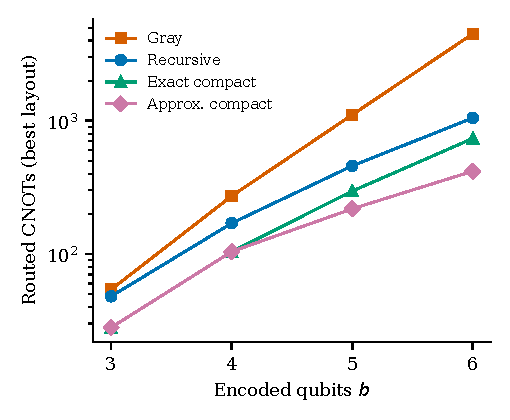
\includegraphics[width=0.62\linewidth]{figures/q2_scaling.pdf}
\caption{Routed nearest-neighbor CNOT counts against encoded qubits $b$ (log scale), each compiler on its own best tested layout. CPU compiler output, not a hardware measurement. The encoded dimension is $2^b$; the ambient Fourier dimension is $2^{2^b-1}$.}\label{fig:q2-scaling}
\end{figure}

\subsection{Phase-contrast protocol}
The primary observable is the phase contrast. For a target shell $n=2^b-1$ and the inputs $\ket{\psi_\pm}=(\ket0\pm\ket1)/\sqrt2$ of the leading shell pair,
\begin{equation}
 C=P(n\mid\psi_-)-P(n\mid\psi_+),
\end{equation}
with ideal value $1$; complete loss of phase information gives $0$. We call this the edge probe. The middle probe uses $\ket{a},\ket{a+1}$ with $a=2^{b-1}$ and the tail probe $a=2^b-2$, with target shell $n-a$ and ideal contrast $1/\sqrt2$. The roster also contains, per probe, the imaginary-phase input $(\ket a+i\ket{a+1})/\sqrt2$, the two basis endpoints (whose average is the incoherent-mixture control), nine preparation-only circuits and the basis-state SPAM controls: 73 circuits at $b=5$ and 58 at $b=6$, 512 shots each, one Sampler V2 job per stage. Every arm in a job uses the same physical chain, the same logical mapping and IBM optimization level 1; the order of circuits is shuffled with a seed that depends on $b$ and the replicate index. Intervals are the pre-registered marginal Hoeffding intervals, of radius $\sqrt{\ln40/512}=0.085$ for a contrast and $0.120$ for a difference of contrasts. They assume independent shots with fixed probabilities, exclude drift and systematic error, and are not adjusted for multiplicity. Positive contrast is not a certificate of process fidelity. Primary comparison: approximate compact against recursive, with exact compact and Gray as controls. Raw counts are used everywhere; no mitigation is applied.

The primary run (replicate 0) used physical chain $[148,149,150,151,152]$ on \texttt{ibm\_kingston}. Replicate 1 repeated the registered $b=5$ roster on the disjoint chain $[67,68,69,78,89]$, selected before any replicate-1 data existed as the lowest-cost calibrated path avoiding the qubits of replicate 0. All three jobs ran under the device calibration of 27 November 2026, 12:56 UTC, so the replicate changes the chain, not the calibration. The $b=6$ stretch run used $[67,68,69,78,89,88]$. IBM charged 14, 14 and 12 QPU seconds for jobs \texttt{dc4oaqqnj2vs73dkf2kg}, \texttt{dc4ock2nj2vs73dkf570} and \texttt{dc4oduinj2vs73dkf74g} (plan hashes beginning \texttt{4c2ef2086e52}, \texttt{13ad51412877} and \texttt{9678e596f7f5}), 40 seconds in total, against estimates of 22.5, 22.5 and 18.3 seconds. The account had 296 of 600 seconds left afterwards.

\begin{table}[htbp]\centering\small
\caption{QPU02, $b=5$: compiled resources on \texttt{ibm\_kingston} (IBM native gates, optimization level 1; identical for every replicate at this $b$). Routed CNOTs are the registered compiler output on the common layout; native two-qubit gates, depth and duration are for the edge phase circuit including preparation. The operator error is the ideal spectral-norm distance from the exact shell transform.}\label{tab:q2res-b5}
\begin{tabular}{lrrrrrr}\toprule Arm & Routed CNOT & Native 2q & 2q depth & Depth & Duration ($\mu$s) & Operator error\\\midrule
Gray & 1122 & 1122 & 1041 & 4509 & 117.7 & 2.2e-14\\
Recursive & 468 & 468 & 434 & 1801 & 48.3 & 4.5e-15\\
Exact compact & 296 & 296 & 271 & 1148 & 31.8 & 4.9e-15\\
Approx. compact & 218 & 218 & 206 & 849 & 24.0 & 1.2e-03\\
\bottomrule\end{tabular}\end{table}

\begin{table}[htbp]\centering\scriptsize\setlength{\tabcolsep}{3pt}
\caption{QPU02, $b=5$, replicate 0: phase contrast $C=P(n\mid\psi_-)-P(n\mid\psi_+)$, 512 shots per circuit, raw counts. Ideal $C$ is 1 (edge) or $1/\sqrt2$ (middle, tail). Intervals are marginal 95\% Hoeffding intervals from finite shots only. $\Delta$ is the contrast minus the recursive arm's, with its interval; TV and $F_H$ are means over the plus, minus and imaginary circuits of each arm (uniform-noise TV reference 0.869).}\label{tab:q2c-b5r0}
\begin{tabular}{llrcrcrr}\toprule Arm & Probe & $C$ & 95\% interval & $C/C_{\rm ideal}$ & $\Delta$ vs recursive & mean TV & mean $F_H$\\\midrule
Gray & edge & 0.012 & [-0.073,+0.097] & 0.012 & -0.004 [-0.124,+0.116] & 0.799 & 0.212\\
Gray & middle & 0.021 & [-0.063,+0.106] & 0.030 & -0.004 [-0.124,+0.116] &  & \\
Gray & tail & 0.023 & [-0.061,+0.108] & 0.033 & -0.047 [-0.167,+0.073] &  & \\
\midrule
Recursive & edge & 0.016 & [-0.069,+0.101] & 0.016 & --- & 0.733 & 0.276\\
Recursive & middle & 0.025 & [-0.059,+0.110] & 0.036 & --- &  & \\
Recursive & tail & 0.070 & [-0.015,+0.155] & 0.099 & --- &  & \\
\midrule
Exact compact & edge & 0.121 & [+0.036,+0.206] & 0.121 & +0.105 [-0.015,+0.226] & 0.642 & 0.385\\
Exact compact & middle & 0.121 & [+0.036,+0.206] & 0.171 & +0.096 [-0.024,+0.216] &  & \\
Exact compact & tail & 0.141 & [+0.056,+0.226] & 0.199 & +0.070 [-0.050,+0.190] &  & \\
\midrule
Approx. compact & edge & 0.189 & [+0.105,+0.274] & 0.189 & +0.174 [+0.054,+0.294] & 0.593 & 0.438\\
Approx. compact & middle & 0.203 & [+0.118,+0.288] & 0.287 & +0.178 [+0.058,+0.298] &  & \\
Approx. compact & tail & 0.211 & [+0.126,+0.296] & 0.298 & +0.141 [+0.021,+0.261] &  & \\
\multicolumn{8}{l}{Preparation-only mean success 0.977; SPAM mean 0.974, min 0.957.}\\
\bottomrule\end{tabular}\end{table}

\begin{table}[htbp]\centering\scriptsize\setlength{\tabcolsep}{3pt}
\caption{QPU02, $b=5$, replicate 1: phase contrast $C=P(n\mid\psi_-)-P(n\mid\psi_+)$, 512 shots per circuit, raw counts. Ideal $C$ is 1 (edge) or $1/\sqrt2$ (middle, tail). Intervals are marginal 95\% Hoeffding intervals from finite shots only. $\Delta$ is the contrast minus the recursive arm's, with its interval; TV and $F_H$ are means over the plus, minus and imaginary circuits of each arm (uniform-noise TV reference 0.869).}\label{tab:q2c-b5r1}
\begin{tabular}{llrcrcrr}\toprule Arm & Probe & $C$ & 95\% interval & $C/C_{\rm ideal}$ & $\Delta$ vs recursive & mean TV & mean $F_H$\\\midrule
Gray & edge & 0.047 & [-0.038,+0.132] & 0.047 & -0.004 [-0.124,+0.116] & 0.789 & 0.218\\
Gray & middle & -0.012 & [-0.097,+0.073] & -0.017 & -0.098 [-0.218,+0.022] &  & \\
Gray & tail & 0.023 & [-0.061,+0.108] & 0.033 & -0.006 [-0.126,+0.114] &  & \\
\midrule
Recursive & edge & 0.051 & [-0.034,+0.136] & 0.051 & --- & 0.692 & 0.324\\
Recursive & middle & 0.086 & [+0.001,+0.171] & 0.122 & --- &  & \\
Recursive & tail & 0.029 & [-0.056,+0.114] & 0.041 & --- &  & \\
\midrule
Exact compact & edge & 0.148 & [+0.064,+0.233] & 0.148 & +0.098 [-0.022,+0.218] & 0.578 & 0.452\\
Exact compact & middle & 0.176 & [+0.091,+0.261] & 0.249 & +0.090 [-0.030,+0.210] &  & \\
Exact compact & tail & 0.238 & [+0.153,+0.323] & 0.337 & +0.209 [+0.089,+0.329] &  & \\
\midrule
Approx. compact & edge & 0.309 & [+0.224,+0.393] & 0.309 & +0.258 [+0.138,+0.378] & 0.498 & 0.540\\
Approx. compact & middle & 0.236 & [+0.151,+0.321] & 0.334 & +0.150 [+0.030,+0.270] &  & \\
Approx. compact & tail & 0.254 & [+0.169,+0.339] & 0.359 & +0.225 [+0.105,+0.345] &  & \\
\multicolumn{8}{l}{Preparation-only mean success 0.964; SPAM mean 0.965, min 0.955.}\\
\bottomrule\end{tabular}\end{table}

\begin{table}[htbp]\centering\small
\caption{QPU02, $b=6$: compiled resources on \texttt{ibm\_kingston} (IBM native gates, optimization level 1; identical for every replicate at this $b$). Routed CNOTs are the registered compiler output on the common layout; native two-qubit gates, depth and duration are for the edge phase circuit including preparation. The operator error is the ideal spectral-norm distance from the exact shell transform.}\label{tab:q2res-b6}
\begin{tabular}{lrrrrrr}\toprule Arm & Routed CNOT & Native 2q & 2q depth & Depth & Duration ($\mu$s) & Operator error\\\midrule
Recursive & 1080 & 1080 & 987 & 4101 & 106.6 & 9.1e-15\\
Exact compact & 736 & 736 & 659 & 2790 & 73.7 & 8.3e-15\\
Approx. compact & 434 & 434 & 400 & 1626 & 43.7 & 1.2e-03\\
\bottomrule\end{tabular}\end{table}

\begin{table}[htbp]\centering\scriptsize\setlength{\tabcolsep}{3pt}
\caption{QPU02, $b=6$, replicate 0: phase contrast $C=P(n\mid\psi_-)-P(n\mid\psi_+)$, 512 shots per circuit, raw counts. Ideal $C$ is 1 (edge) or $1/\sqrt2$ (middle, tail). Intervals are marginal 95\% Hoeffding intervals from finite shots only. $\Delta$ is the contrast minus the recursive arm's, with its interval; TV and $F_H$ are means over the plus, minus and imaginary circuits of each arm (uniform-noise TV reference 0.925).}\label{tab:q2c-b6r0}
\begin{tabular}{llrcrcrr}\toprule Arm & Probe & $C$ & 95\% interval & $C/C_{\rm ideal}$ & $\Delta$ vs recursive & mean TV & mean $F_H$\\\midrule
Recursive & edge & -0.006 & [-0.091,+0.079] & -0.006 & --- & 0.922 & 0.069\\
Recursive & middle & -0.020 & [-0.104,+0.065] & -0.028 & --- &  & \\
Recursive & tail & -0.010 & [-0.095,+0.075] & -0.014 & --- &  & \\
\midrule
Exact compact & edge & -0.002 & [-0.087,+0.083] & -0.002 & +0.004 [-0.116,+0.124] & 0.891 & 0.096\\
Exact compact & middle & 0.000 & [-0.085,+0.085] & 0.000 & +0.020 [-0.101,+0.140] &  & \\
Exact compact & tail & -0.008 & [-0.093,+0.077] & -0.011 & +0.002 [-0.118,+0.122] &  & \\
\midrule
Approx. compact & edge & 0.020 & [-0.065,+0.104] & 0.020 & +0.025 [-0.095,+0.145] & 0.883 & 0.110\\
Approx. compact & middle & 0.004 & [-0.081,+0.089] & 0.006 & +0.023 [-0.097,+0.143] &  & \\
Approx. compact & tail & -0.002 & [-0.087,+0.083] & -0.003 & +0.008 [-0.112,+0.128] &  & \\
\multicolumn{8}{l}{Preparation-only mean success 0.965; SPAM mean 0.956, min 0.938.}\\
\bottomrule\end{tabular}\end{table}



\begin{figure}[htbp]\centering
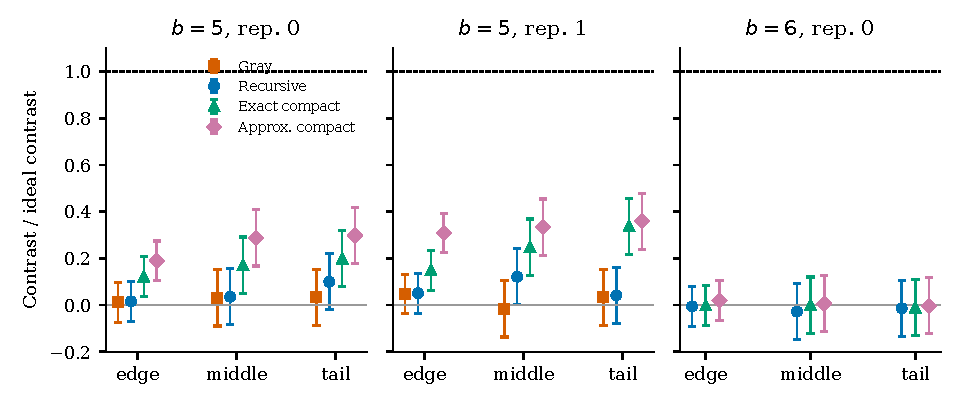
\includegraphics[width=0.98\linewidth]{figures/q2_contrast.pdf}
\caption{Phase contrast divided by its ideal value for each arm and probe (95\% Hoeffding intervals, finite shots only). Dashed line: ideal. The $b=5$ runs on two disjoint chains are on the left and centre; the $b=6$ run is on the right. Ambient Fourier dimensions are $2^{31}$ and $2^{63}$.}\label{fig:q2-contrast}
\end{figure}
\begin{figure}[htbp]\centering
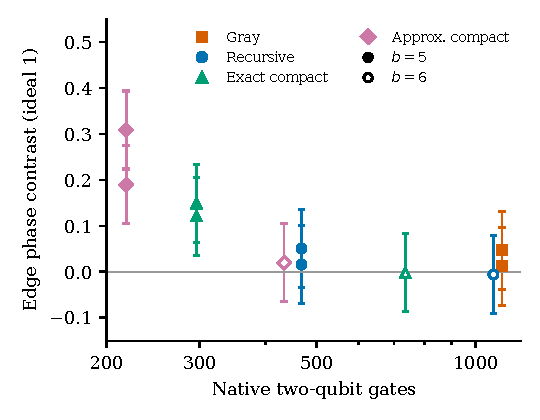
\includegraphics[width=0.62\linewidth]{figures/q2_contrast_vs_gates.pdf}
\caption{Edge phase contrast against native two-qubit gate count for all arms and stages (filled: $b=5$, both replicates; open: $b=6$). Error bars as in Figure~\ref{fig:q2-contrast}.}\label{fig:q2-gates}
\end{figure}

\subsection{Hardware results}
\paragraph{Five encoded qubits.} The compiled circuits keep the registered CNOT counts, 1,122, 468, 296 and 218 native two-qubit gates for Gray, recursive, exact compact and approximate compact (Table~\ref{tab:q2res-b5}); schedule durations are $117.7$, $48.3$, $31.8$ and $24.0\,\mu$s. Phase contrast is small for every arm (Table~\ref{tab:q2c-b5r0}, \ref{tab:q2c-b5r1}, Figure~\ref{fig:q2-contrast}). On the edge probe the contrasts of Gray and recursive circuits are $0.012$ and $0.016$ in replicate 0 and $0.047$ and $0.051$ in replicate 1, indistinguishable from zero. The exact compact circuit gave $0.121$ and $0.148$, and the approximate compact circuit $0.189$ and $0.309$, so $19\%$ and $31\%$ of the ideal contrast. Averaged over the two replicates the edge contrasts are $0.030$ (Gray), $0.034$ (recursive), $0.135$ (exact compact) and $0.249$ (approximate compact). Against the recursive arm, the approximate compact circuit improves the edge contrast by $+0.174$ (interval $[+0.054,+0.294]$) in replicate 0 and $+0.258$ ($[+0.138,+0.378]$) in replicate 1. Its middle and tail differences are positive in both replicates and all six intervals exclude zero. The exact compact circuit also has a positive difference in every probe and replicate ($+0.07$ to $+0.21$), but only the replicate-1 tail interval ($+0.209$, $[+0.089,+0.329]$) excludes zero. The Gray circuit does not differ from the recursive one (differences from $-0.098$ to $-0.004$, all intervals contain zero). The two replicates differ by $0.12$ for the approximate edge contrast, as large as the shot-noise half-width of a difference, so we cannot say whether the chain matters.

The distribution-level metrics point the same way. The mean total variation distance over the plus, minus and imaginary circuits was $0.799/0.789$ (Gray), $0.733/0.692$ (recursive), $0.642/0.578$ (exact) and $0.593/0.498$ (approximate) for replicates 0 and 1, with a uniform-noise reference of $0.869$; the mean Hellinger fidelities were $0.212/0.218$, $0.276/0.324$, $0.385/0.452$ and $0.438/0.540$. Even the best arm is far from the ideal distribution. Preparation-only circuits succeeded with probability $0.977$ and $0.964$ on average and basis-state SPAM controls $0.974$ and $0.965$ (minimum $0.955$), so state preparation and readout are not what removes the contrast. The midpoint-versus-mixture and imaginary-versus-mixture total variation distances are between $0.07$ and $0.20$ for every arm, including arms whose contrast is zero, so they are dominated by sampling and noise and give no independent evidence of phase sensitivity.

\paragraph{Six encoded qubits: saturated.} The $b=6$ circuits have 1,080, 736 and 434 native two-qubit gates (recursive, exact, approximate; Table~\ref{tab:q2res-b6}). All nine contrasts lie within $\pm0.02$ of zero (Table~\ref{tab:q2c-b6r0}), every approximate-minus-recursive difference has an interval containing zero, and the mean total variation distances ($0.92$, $0.89$, $0.88$) are close to the uniform-noise value of $0.925$. Preparation-only controls succeeded with probability $0.965$ and SPAM controls with $0.956$ on average, so the loss comes from the transform circuits. The six-qubit stretch therefore showed no phase contrast for any arm and does not support a hardware benefit at this size. For comparison, the five-qubit recursive circuit, with $468$ native gates, had edge contrasts of only $0.016$ and $0.051$, and the six-qubit approximate circuit, with $434$, gave $0.020$. Edge contrast against native gate count (Figure~\ref{fig:q2-gates}) is consistent with a signal that nearly disappears at a few hundred two-qubit gates on this device, but three stages with different arms do not establish a functional dependence.

\paragraph{Limits.} These data come from one backend, one calibration and one 512-shot sample per circuit. The replicate changes the physical chain but not the calibration, the five-qubit replicates share the compiled circuits and the roster, and the nine contrasts of a stage use shared hardware conditions, so they are not independent. The intervals are shot-only. Optimization level 1 was applied to all arms, and a different transpiler setting could change the relative gate counts. The contrast of the best arm is at most $0.36$ of the ideal value, so the experiment does not demonstrate a coherent Fourier transform in the sense of a high-fidelity circuit; it shows that after exact or bounded-error compaction a measurable fraction of the phase contrast survives where the uncompacted recursive and Gray circuits show little or none. All statements concern the transform on the unit-invariant subspace of dimension $2^b$. They do not establish a general QFT acceleration or a quantum computational advantage, the cost of preparing the encoded inputs is excluded, and the classical simulation of the shell dynamics in $O(2^b)$ amplitudes remains available. The four-qubit anchor with compact arms was not run, and the six-qubit Gray circuit was compiled only on CPU.

\section{Next steps toward a submission}
A submission should add a targeted literature review of the binary recursive identity and circuit complexity of Ramanujan or supercharacter transforms; the normalized orbit matrix is already known. Extending the recursion to arbitrary shell counts and quantifying approximate symmetry for realistic input ensembles would broaden its scope. A controlled-QFT and phase-oracle study should include synthesis costs and comparisons against modern approximate QFT circuits, along with the direct hierarchical baseline. The hardware pilots of Sections~\ref{sec:hardware} and~\ref{sec:compact} should be repeated across calibrations with native-gate optimization of every arm, a four-qubit anchor with the compact circuits, and coherent spectral-phase sandwiches; six encoded qubits need substantially fewer native two-qubit gates before phase contrast is measurable on this device. Together with the ideal simulation receipts, it supports a mathematical and engineering draft; the measured accuracy results are inconclusive, and the draft makes no claim of general hardware advantage or priority.

\begin{thebibliography}{9}\small
\bibitem{fowler} C. F. Fowler, S. R. Garcia, G. Karaali, ``Ramanujan sums as supercharacters,'' \emph{Ramanujan Journal}; preprint \href{https://arxiv.org/abs/1201.1060}{arXiv:1201.1060} (2012).
\bibitem{brumbaugh} J. L. Brumbaugh et al., ``Supercharacters, exponential sums, and the uncertainty principle,'' \emph{Journal of Number Theory} 144, 151--175 (2014), \href{https://doi.org/10.1016/j.jnt.2014.04.019}{doi:10.1016/j.jnt.2014.04.019}.
\bibitem{nam} Y. Nam, Y. Su, D. Maslov, ``Approximate quantum Fourier transform with $O(n\log n)$ T gates,'' \emph{npj Quantum Information} 6, 26 (2020), \href{https://doi.org/10.1038/s41534-020-0257-5}{doi:10.1038/s41534-020-0257-5}.
\bibitem{shah} R. Shah, ``A Faster Quantum Fourier Transform,'' preprint \href{https://arxiv.org/abs/2501.12414}{arXiv:2501.12414} (2025).
\bibitem{bendikov} A. Bendikov, P. Krupski, ``On the spectrum of the hierarchical Laplacian,'' \emph{Potential Analysis} 41, 1247--1266 (2014), \href{https://doi.org/10.1007/s11118-014-9409-6}{doi:10.1007/s11118-014-9409-6}.
\bibitem{grover} L. Grover, T. Rudolph, ``Creating superpositions that correspond to efficiently integrable probability distributions,'' \href{https://arxiv.org/abs/quant-ph/0208112}{arXiv:quant-ph/0208112} (2002).
\bibitem{mottonen} M. M\"ott\"onen et al., ``Transformation of quantum states using uniformly controlled rotations,'' \href{https://arxiv.org/abs/quant-ph/0407010}{arXiv:quant-ph/0407010} (2004).
\bibitem{zuniga} W. A. Z\'u\~niga-Galindo, N. P. Mayes, ``p-Adic quantum mechanics, infinite potential wells, and continuous-time quantum walks,'' \emph{Reviews in Mathematical Physics} 38, 2550027 (2026), \href{https://arxiv.org/abs/2410.13048}{arXiv:2410.13048}.
\end{thebibliography}
\end{document}
